Now we will study several different methodologies for the creation and managing of enormous geometric models. At first we will see some methodological instruments which are at the basis of a powerful library for geometric modeling developed at the \textit{Computational and Visual Design} laboratory in the Roma Tre University: \textbf{LAR}. It is essentially based in algebraic topology techniques, which will be introduced here.\\

As a consequence, the chapter will first go through a general overview of the topology field, then it will study in detail the LAR representation schema and some interesting topological operators

\section{Fundamentals of topology}\label{sec21:topologicalAlgebra}

In this section we will give a general overview of the \textbf{topology} field. In mathematics, topology is concerned with the properties of spaces that are preserved under \textbf{continuous deformations}, such as \textit{stretching} and \textit{bending}, but \textbf{not} \textit{tearing} and \textit{gluing}. Topology comes from geometry and set theory, and the first theorems of the field come from the Euler's \textit{Seven Bridges of Königsberg Problem} and from the \textit{Polyhedron Formula} (which we have already seen in Chapter~\ref{sec14:MemoryReq}) . It has many subfields:
\begin{itemize}
 \item \textbf{General topology}: covers the foundational aspects of topology and investigates properties of topological spaces and concepts inherent to topological spaces
 \item \textbf{Algebraic topology}: tries to measure degrees of connectivity using algebraic constructs such as homology and homotopy groups
 \item \textbf{Differential topology}: deals with differentiable functions on differentiable manifolds. It is closely related to differential geometry
 \item \textbf{Geometric topology}: studies manifolds and their embeddings in other manifolds. A particularly active area is low-dimensional topology which studies manifolds of four or fewer dimensions
\end{itemize}

Now we can study in detail this field giving some definitions.
First of all from \cite{Kosniowski} we learn that a \textbf{topological space} is a set satisfying three properties

\begin{definition}[Topological space]
 Let $X$ be a set and let $\mathcal{U}$ be a collection of subsets of $X$ satisfying:
 \begin{enumerate}
  \item $\emptyset \in \mathcal{U}$, $X \in \mathcal{U}$
  \item the intersection of two members of $\mathcal{U}$ is in $\mathcal{U}$
  \item the union of any number of members of $\mathcal{U}$ is in $\mathcal{U}$
 \end{enumerate}
 Such a collection $\mathcal{U}$ of subsets of $X$ is called a \textbf{topology} for $X$. The set $\mathcal{U}$ together with $X$ is called a \textbf{topological space} and is denoted by $(X,\mathcal{U})$ which is often abbreviated to $T$ or just $X$. The members $U \in \mathcal{U}$ are called the \textbf{open sets\footnote{Intuitively, we say that a set is \textit{open} if we can move slightly in every direction from every point of the set without leaving it. The complementary of an open set is a \textbf{closed set}}} of $T$. Elements of $X$ are called \textbf{points} of $T$
\end{definition}

A typical example of topological space is the \textbf{metric space}:

\begin{definition}[Metric space]
 A \textbf{metric space} is an ordered pair $(M, d)$ where $M$ is a set and $d$ is a metric on $M$, i.e., a function $d \colon M \times M \to \mathbb{R}$ such that for any $x,y,z \in M$ the following holds:
 \begin{enumerate}
  \item $d(x,y) \ge 0$
  \item $d(x,y) = 0 \iff x = y$
  \item $d(x,y) = d(y,x)$
  \item $d(x,z) \le d(x,y) + d(y,z)$
 \end{enumerate}
\end{definition}

The most famous example of a metric space is the \textbf{Euclidean space} (consequently a topological space). So every object contained in a plane or in a space (such as polygons and fractals) is a topological space\\

As we have seen above, topology studies spaces but also the deformations applied. So we can introduce the notion of \textbf{continuous functions}:

\begin{definition}[Continuous function]
 A function $f \colon X \rightarrow Y$ between two topological spaces is said to be \textbf{continuous} if for every open set $U$ of $Y$ the inverse image $f^{-1}(U)$ is open in $X$
\end{definition}

For example the identity function and the constant function are continuous functions. When two topological spaces are equivalent it is said there is an \textbf{homeomorphism}:

\begin{definition}[Homeomorphism]
 Let $X$ and $Y$ be topological spaces. We say that $X$ and $Y$ are \textbf{homeomorphic} if inverse continuous functions $f \colon X \rightarrow Y$, $g \colon Y \rightarrow X$ exist. We write $X \cong Y$ and say that $f$ and $g$ are \textbf{homeomorphisms} between $X$ and $Y$
\end{definition}

An equivalent definition is:
\begin{definition}[Homeomorphism(2)]
 A function $f \colon X \rightarrow Y$ between two topological spaces $(X,T_{x})$ and $(Y, T_{y})$ is called a \textbf{homeomorphism} if it has the following properties:
 \begin{enumerate}
  \item $f$ is a bijection
  \item $f$ is continuous
  \item the inverse function $f^{-1}$ is continuous (f is an open mapping)
 \end{enumerate}

\end{definition}

In other words, according to this definition, we have a bijective function between $X$ and $Y$ which links the open sets of $X$ with the open sets of $Y$. For example we can say that a square and a circle are \textit{homeomorphic} and so a mug and a torus, because we can define a function to map one space to the other. Thus, using homeomorphism we can define new topological spaces from known ones.\\

\begin{figure}[htb] %  figure placement: here, top, bottom
   \centering
   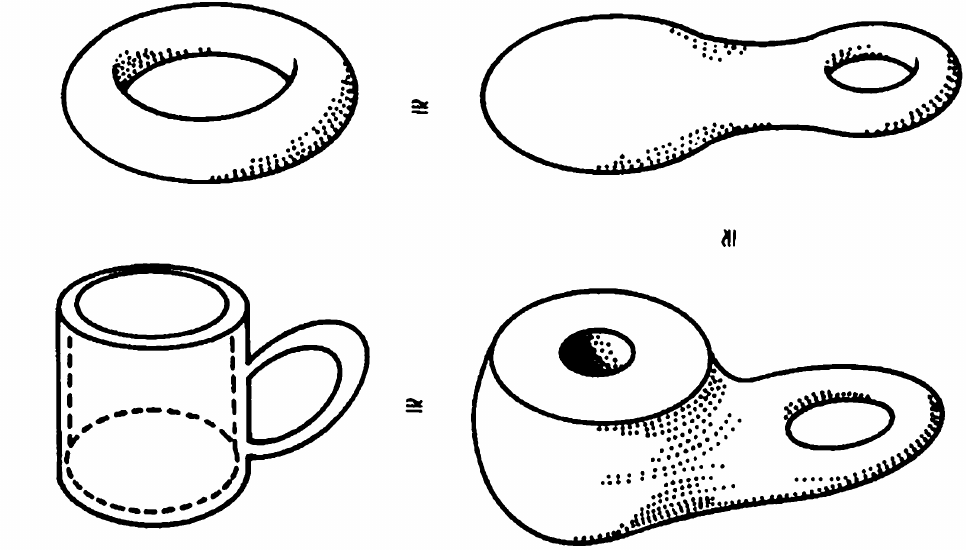
\includegraphics[width=0.45\linewidth]{images/mugTorus.png}
   \caption[Homeomorphisms between a mug and a torus]{Homeomorphisms between a mug and a torus. Image taken from~\cite{Kosniowski}}
   \label{fig:homeomorphisms}
\end{figure}

Now we can introduce another important definition for the construction of a topological space from a given one:

\begin{definition}[Quotient space]
 Suppose that $f \colon X \rightarrow Y$ is a surjective mapping from a topological space $X$ onto a set $Y$. The \textbf{quotient topology} on $Y$ with respect to $f$ is the family $\mathcal{U}_{f} = \{ U; f^{-1}(U)$ is open in $X \}$
\end{definition}

\cite{Kosniowski} has a good example of a quotient space. We can consider the space:
\begin{math}
 C = \{ (x,y,z) \in \mathbb{R}^{3}; x^{2} + y^{2} = 1, |z| \leq 1 \}
\end{math}

which represents a cylinder. Let $M$ be the set of unordered pairs of points in $C$ of the form $\{p,-p\}$, i.e:
\begin{math}
 M = \{ \{p,-p\}; p \in C \}
\end{math}

Since we have a natural surjective map from $C$ to $M$ we can give $M$ the quotient topology; the result is called a \textbf{Mobius strip}.

\begin{figure}[htb] %  figure placement: here, top, bottom
   \centering
   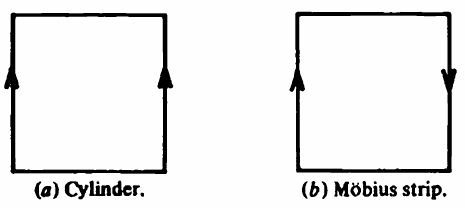
\includegraphics[width=0.65\linewidth]{images/mobiusStripCylinder.png}\\
   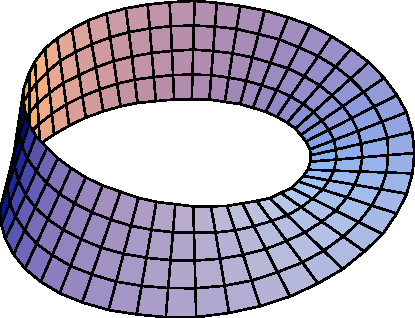
\includegraphics[width=0.35\linewidth]{images/MobiusStrip.pdf}
   \caption[Relationship between Mobius strip and a cylinder]{(\textit{First row}) Flat view of a Mobius strip and a cylinder. (\textit{Second row}) three-dimensional view of a Mobius strip. Images taken from \cite{Kosniowski} and Wikipedia}
   \label{fig:MobiusCylinder}
\end{figure}

At this point, we have seen the main definitions for topology and different ways to generate topological spaces. In the next subsections we will study some interesting topological spaces which will be used in later parts

\subsection{Chain complexes}

Now we can introduce a very important construct of the algebraic topology the \textbf{chain complexes}. They are algebraic means of representing the relationships between \textit{cycles} and \textit{boundaries} in various dimensions of a topological space. To fully understand the theory behind chain complexes we should introduce other interesting definitions first:

\begin{definition}[Standard n-simplex]
 The \textbf{standard n-simplex} $\Delta_{n}$ is defined to be the following subspace of $\mathbb{R}^{n+1}$:\\
 $\Delta_{n} = \{ x=(x_{0},x_{1},\dots,x_{n}) \in \mathbb{R}^{n+1}; \displaystyle\sum_{i=0}^{n} x_{i} = 1, x_{i} \geq 0, i = 0,1,\dots,n \}$\\
 The points $v_{0} = (1,0,\dots,0), v_{1} = (0,1,0,\dots,0),\dots, v_{n} = (0,0,\dots,0,1)$ are called the vertices of $\Delta_{n}$
\end{definition}

\begin{figure}[htb] %  figure placement: here, top, bottom
   \centering
   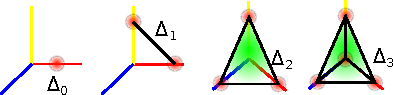
\includegraphics[width=0.80\linewidth]{images/standardSimplices.pdf}
   \caption[Examples of standard n-simplices]{Examples of standard simplices. $\Delta_{0}$ is a point, $\Delta_{1}$ is a line, $\Delta_{2}$ is a triangle and $\Delta_{3}$ is a tetrahedron}
   \label{fig:standardSimplex}
\end{figure}

\begin{definition}[Singular n-simplex]
 Let $X$ be a topological space. A \textbf{singular n-simplex} in $X$ is a continuous map $\varphi \colon \Delta_{n} \rightarrow X$
\end{definition}

So a singular 0-simplex is a point in $X$, while a singular 1-simplex is a path in $X$.

\begin{figure}[htb] %  figure placement: here, top, bottom
   \centering
   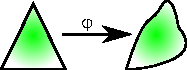
\includegraphics[width=0.35\linewidth]{images/singularsimplex.pdf}
   \caption[A singular n-simplex]{A singular n-simplex.}
   \label{fig:singularSimplex}
\end{figure}


Now we can define the \textbf{singular n-chain}:

\begin{definition}[Singular n-chain]
 A singular n-chain in $X$ is an expression of the form $\displaystyle\sum_{j  \in J} n_{j} \varphi_{j}$ where $\{ \varphi_{j}; j \in J \}$ is the collection of all singular n-simplexes in $X$ (with $J$ some indexing set) and $n_{j} \in \mathbb{Z}$ with only a finite number of $\{ n_{j}; j \in J \}$ being non-zero
\end{definition}

In other words we can say that a simplicial k-chain is a linear combination of k-simplices.
The set $S_{n}(X)$ of singular n-chains in $X$ form an abelian group\footnote{We say that an abelian group is a group where its binary operation is commutative} with the addition defined by $\sum n_{j} \varphi_{j} + \sum m_{j} \varphi_{j} = \sum(n_{j} + m_{j}) \varphi_{j}$. This group has extremely interesting properties which we will exploit in the following parts and that makes it a fundamental construct for LAR library.

Now that we have a definition of a chain complex, we can also define the \textbf{cochain complex}:

\begin{definition}[Singular n-cochain]
Given a topological space $X$ and an abelian group $G$, we define the group $C^{n}(X;G)$ of \textbf{singular n-cochains with coefficients in G} to be the dual group of the singular chain group $C_{n}(X)$. Thus an n-cochain $\varphi \in C^{n}(X;G)$ assigns to each singular n-simplex $\sigma \colon \Delta_{n} \rightarrow X$ a value $\varphi(\sigma) \in G$. Since the singular n-simplices form a basis for $C_{n}(X)$, these values can be chosen arbitrarily hence n-cochains are exactly equivalent to functions from singular n-simplices to $G$.
\end{definition}

This definition is taken from~\cite{Hatcher}.
From a computer science point of view, cochains offer a mechanism for representation of quantities associated with combinatorial and discrete representations. As a consequence, we can use them to represent physical properties for our domain.


\subsection{Cell complexes}

Another fundamental construct of algebraic topology, are \textbf{cell complexes}, which provide a useful procedure for the construction of a topological space. As we can see in~\cite{Hatcher} we can use the following procedure:
\begin{enumerate}
 \item Start with a discrete set $X^{0}$, whose points are referred to as \textbf{0-cells}
 \item Inductively, form the \textbf{n-skeleton} $X^{n}$ from $X^{n - 1}$ by attaching n-cells $e^{n}_{\alpha}$ via maps $\varphi_{\alpha} \colon S^{n-1} \rightarrow X^{n-1}$. This means that $X^{n}$ is the quotient space of the disjoint union $X^{n-1} \coprod_{\alpha}D^{n}_{\alpha}$ of $X^{n-1}$ with a collection of n-disks $D^{n}_{\alpha}$ under the identifications $x \sim  \varphi_{\alpha}(x)$ for $x \in \partial D^{n}_{\alpha}$\footnote{$\partial D^{n}_{\alpha}$ is the boundary of the n-disk as we will see in section~\ref{sec21:topologicalOperators}}. Thus as a set, $X^{n} = X^{n-1}\coprod_{\alpha}e^{n}_{\alpha}$ is an open-disk.
 \item One can either stop this inductive process at a finite stage, setting $X = X^{n}$ for some $x < \infty$, or one can continue indefinitely, setting $X = \bigcup_{n}X^{n}$. In the latter case $X$ is given the \textbf{weak topology}: A set $A \subset X$ is open (or closed) iff $A \cap X^{n}$ is open (or closed) in $X^{n}$ for each $n$
\end{enumerate}

A space $X$ constructed in this way is called a \textbf{cell complex} or \textbf{CW complex}. If $X = X^{n}$ for some $n$, then $X$ is said to be finite-dimensional, and the smallest such $n$ is the \textbf{dimension} of $X$, the maximum dimension of cells of X. We could prove that a n-dimensional cell is homeomorphic to a \textit{n-dimensional ball}\\

In addition, \cite{Hatcher} gives us interesting examples of cell complexes. For example a 1-dimensional cell complex $X = X^{1}$ is a \textbf{graph} in algebraic topology. It consists of vertices (the 0-cells) to which edges (the 1-cells) are attached. The two ends of an edge can be attached to the same vertex.\\
Another example consists in considering the sphere $S^{n}$ which is a cell complex with just two cells. These cells are $e^{0}$ and $e^{n}$, where the n-cell is attached by the constant map $S^{n-1} \rightarrow e^{0}$. This is equivalent to considering $S^{n}$ as the quotient space $D^{n}/\partial D^{n}$.\\

We can also give the following definition:

\begin{definition}[Subcomplex]
A \textbf{subcomplex} of a cell complex $X$ is a closed subspace $A \subset X$ that is a union of cells of $X$. Since $A$ is closed, the characteristic map of each cell in $A$ has image contained in $A$, and in particular the image of the attaching map of each cell in $A$ is contained in $A$, so $A$ is a cell complex in its own right. A pair $(X,A)$ consisting of a cell complex $X$ and a subcomplex $A$ will be called a \textbf{CW pair}.
\end{definition}

According to \cite{Hatcher}, we can also define various operations on cell complexes. We have:
\begin{description}
 \item \textbf{Products}. If $X$ and $Y$ are cell complexes, then $X \times Y$ has the structure of a cell complex where cells are the products $e^{m}_{\alpha} \times e^{n}_{\beta}$ where $e^{m}_{\alpha}$ ranges over the cells of $X$ and $e^{n}_{\beta}$ over the cells of $Y$
 \item \textbf{Quotients}.  If $(X, A)$ is a CW pair consisting of a cell complex $X$ and a subcomplex $A$, then the quotient space $X/A$ inherits a cell complex structure from $X$. The cells of $X/A$ are the cells of $X - A$ plus one new 0-cell, which is the image of $A$ in $X/A$. For a cell $e^{n}_{\alpha}$ of $X-A$ attached by $\varphi_{\alpha} \colon S^{n-1} \rightarrow X^{n-1}$, the attaching map for the corresponding cell in $X/A$ is the composition $S^{n-1} \rightarrow X^{n-1} \rightarrow X^{n-1}/A^{n-1}$
 \item \textbf{Suspension}. For a space $X$, the suspension $SX$ is the quotient of $X \times I$ obtained by collapsing $X \times \{0\}$ to one point and $X \times \{1\}$ to another point.
 \item \textbf{Join}. Given $X$ and a second space $Y$, one can define the space of all line segments joining points in $X$ to points in $Y$. This is the join $X \ast Y$, the quotient space of $X \times Y \times I$ under the identifications $(x, y_{1}, 0) \sim (x, y_{2}, 0)$ and $(x_{1}, y, 1) \sim (x_{2}, y, 1)$. Thus we are collapsing the subspace $X \times Y \times \{0\}$ to $X$ and $X \times Y \times \{1\}$ to $Y$.
 \item \textbf{Wedge Sum}. Given spaces $X$ and $Y$ with chosen points $x_{0} \in X$ and $y_{0} \in Y$, then the wedge sum $X \vee Y$ is the quotient of the disjoint union $X \sqcup Y$ obtained by identifying $x_{0}$ and $y_{0}$ to a single point.
 \item \textbf{Smash Product}. Inside a product space $X \times Y$ there are copies of $X$ and $Y$, namely $X \times \{y_{0}\}$ and $\{x_{0}\} \times Y$ for points $x_{0} \in X$ and $y_{0} \in Y$. These two copies of $X$ and $Y$ in $X \times Y$ intersect only at the point $(x_{0}, y_{0})$, so their union can be identified with the wedge sum $X \vee Y$. The smash product $X \wedge Y$ is then defined to be the quotient $X \times Y/X \vee Y$
\end{description}
In Figure~\ref{fig:cellOperations} there is a graphical representation of all these operations.

\begin{figure}[htbp] %  figure placement: here, top, bottom
   \centering
   (a)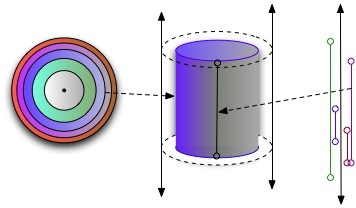
\includegraphics[width=0.50\linewidth]{images/productTopology.jpg}\hfill
   (b)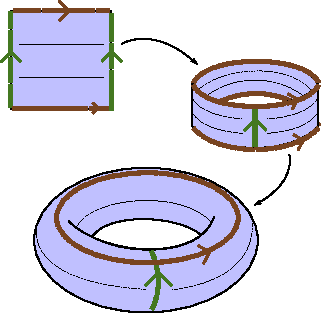
\includegraphics[width=0.23\linewidth]{images/quotientTopology.pdf}\hfill
   (c)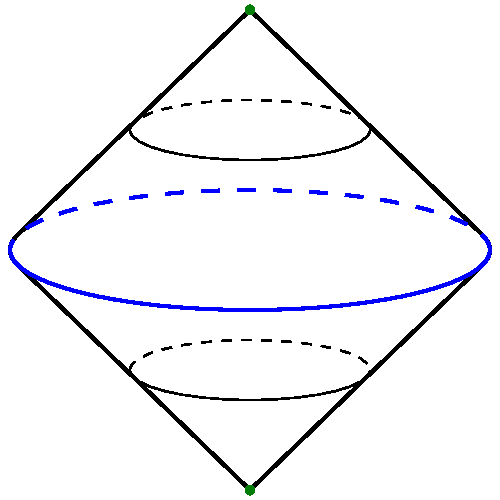
\includegraphics[width=0.30\linewidth]{images/suspensionTopology.pdf}\\
   (d)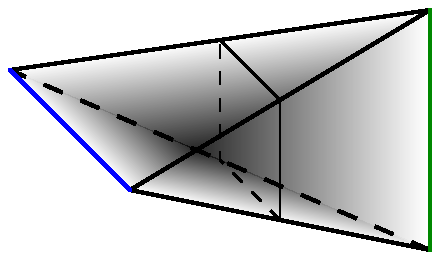
\includegraphics[width=0.30\linewidth]{images/joinTopology.pdf}\hfill
   (e)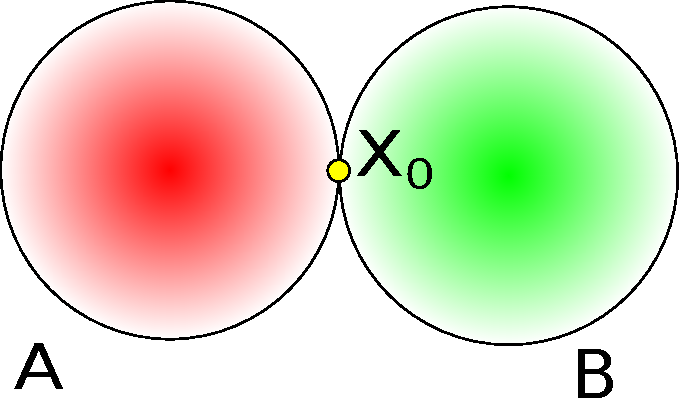
\includegraphics[width=0.30\linewidth]{images/wedgeSum.pdf}\\
   (f)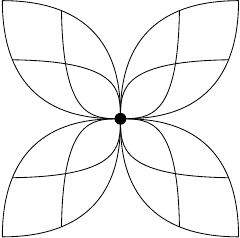
\includegraphics[width=0.30\linewidth]{images/smashProduct.png}\\
   \caption[Operations on cell complexes]{Operations on cell complexes.\\ (a) A product topology. How we can see, a cylinder can be obtained with a product between a circle and a line. Image taken from \href{http://scienceblogs.com/goodmath/2006/09/21/topological-products/}{scienceblogs.com}\\ (b) A quotient topology. Intuitively we have a quotient topology when we glue spaces points together. For example we can obtain a torus by gluing opposite sides of a square. Image taken from \href{http://mathroughguides.wikidot.com/article:point-set-topology}{mathroughguides.wikidot.com}\\ (c) A suspension topology. The original space is in blue and the collapsed end points are in green. Image taken from Wikipedia.\\ (d) Geometric join of two line segments. The original spaces are in blue and green. The join is a three-dimensional solid in black. Image taken from Wikipedia\\ (e) A wedge sum topology obtained by attaching two circumferences by a point\\ (f) Smash product. In this example we build a smash product starting from two segments. The product topology produces a square and then the vertical and the horizontal lines are collapsed to a point. Image taken from \href{http://www.math.ntnu.no/~stacey/Seminars/chern.html}{www.math.ntnu.no}}
   \label{fig:cellOperations}
\end{figure}

\section{LAR representation schema}\label{sec21:LAR}

As stated in \cite{DiCarlo} (and also in the first chapters of this work), present-day computational problems in science and technology must deal with increasingly complex geometric information. The evolution of 3D geometric representations can be generally understood in terms of graph-based data structures representing one of several possible cell complexes partitioning either the boundary or the interior of the represented model. However, we can make a lot of assumptions about cell complexes and graph representations, so standardization seem difficult to reach. Thus the specialized data structures that have been used since now, are no longer adequate to deal with these problems.\\

\cite{DiCarlo} provides a solution to these problems with a new representation schema which supports all topological constructions and queries useful in typical cellular decomposition of space: \textbf{LAR}. Formally, LAR uses the standard definitions of the mod-2 cell complexes. So we have \textit{n-chains} which are sets of \textit{n-cells}. The standard basis of the $\mathbb{Z}_{2}$-linear space $C_{d}$ of n-chains is provided by singletons of n-cells; each n-cell is represented by a map $C_{n} \rightarrow \mathbb{Z}_{2}C_{0}$, i.e. by a row of a binary characteristic matrix $M_{n}$. Obviously, each n-chain in $C_{n}$ can be generated by a $(\mathbb{Z}_{2})$-linear combination of $M_{n}$ rows. This formulation can be extended to n-cochains that represent any possible field over the chains.\\

\begin{figure}[htb] %  figure placement: here, top, bottom
   \centering
   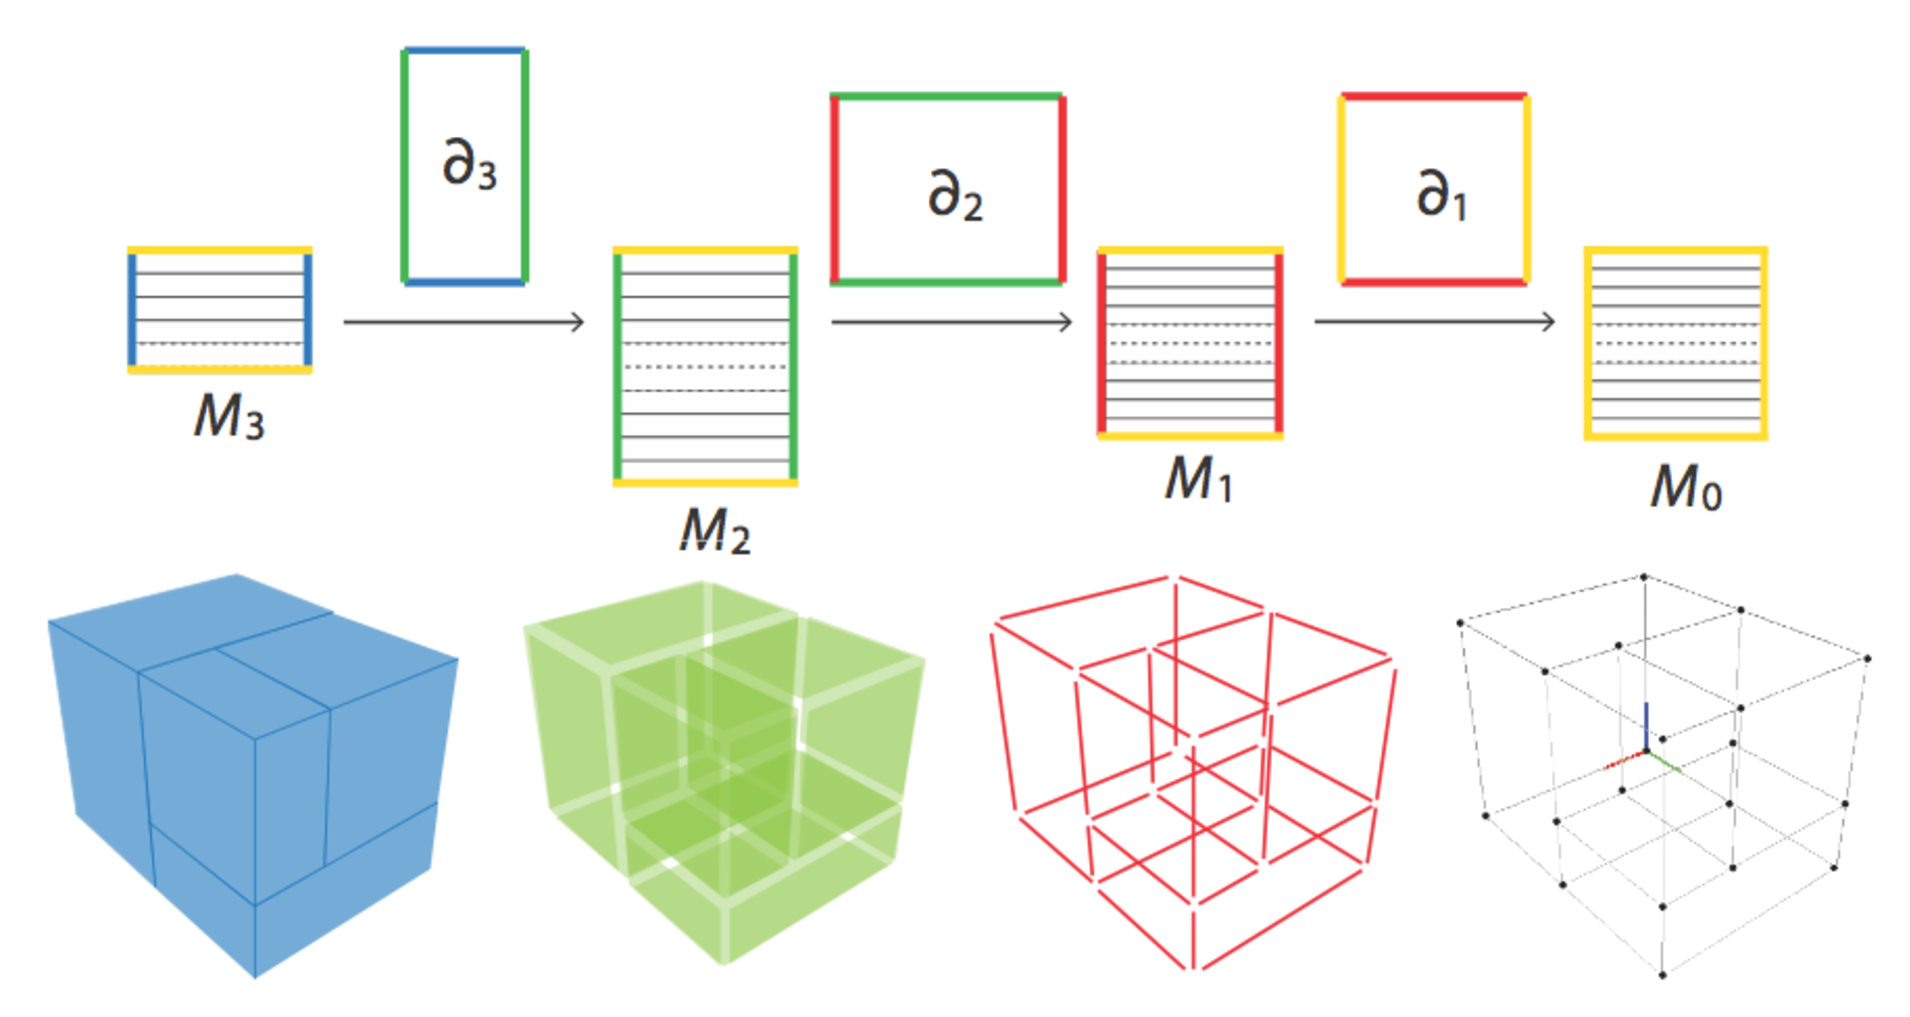
\includegraphics[width=0.75\linewidth]{images/larcomplex.pdf}\\
   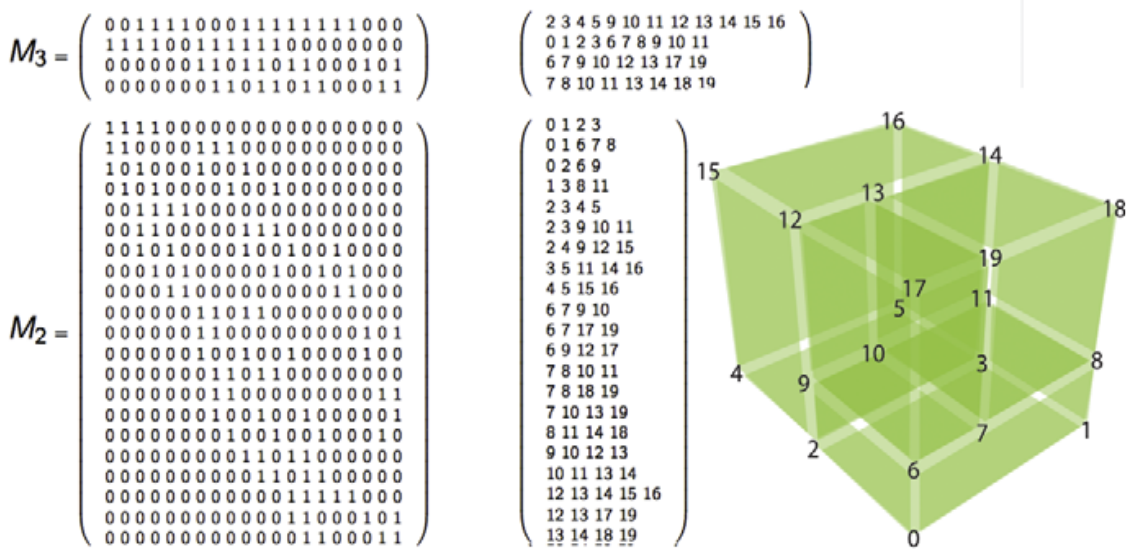
\includegraphics[width=0.85\linewidth]{images/larRepresentation.png}
   \caption[LAR representation schema]{LAR representation schema. We can see the relationship between chains of different dimensions and how to represent them using a characteristic matrix. Images taken from \cite{DiCarlo}}
   \label{fig:larRepresentation}
\end{figure}

Figure~\ref{fig:larRepresentation}, points out that characteristic matrices are very sparse for actual chain complexes, so they can be represented in the \textbf{Compressed Sparse Row} (CSR) format in order to save space. This format is widely used in computer science, and consists in using three one-dimensional arrays. The first one save the non-zero values as they are traversed in a row-wise fashion, while the second stores the columns indices of the values. The last one stores the locations of the values array that start a row. Moreover, if we have a binary matrix we can safely delete the first array, as the non-zero value can only be $1$. In addition this data structure is faster than a traditional one, because the \textbf{sparse matrix-vector multiplication} (SpMV) is linear in the size of the output.\\

Now we can deeply study the LAR representation from a formal point of view using concepts from \cite{DiCarlo}. First of all we need to consider a cellular complex $\Lambda(X)$ such that $X = \Lambda_{0} \cup \dots \cup \Lambda_{d}$. We can define $M_{p} \in \mathbb{Z}_{2}^{m\times n} (0\leq p \leq d)$ as the characteristic matrices, with number of rows equal to the number of p-cells and number of columns equal to the number of 0-cells:
\begin{equation}
 m = k_{p} = \#\Lambda_{p}, \; \; \; \; \; \; \; \; n = k_{0} = \#\Lambda_{0}
\end{equation}

Each $m_{ij} \in M_{p}$ tells us whether the vertex $v_{j} \in \Lambda_{0}$ is contained on the boundary of the cell $\lambda_{i} \in \Lambda_{p}$ or not. So the LAR schema is a map from a mathematical model of a solid to its computer representation:
\begin{equation}
 LAR \colon \mathbb{C}h(\Lambda(X)) \rightarrow (M_{p})^{d}_{p=1}
\end{equation}

So we can have the following definition from \cite{DiCarlo}:
\begin{definition}[LAR representation]
 $LAR$ represents chain complexes $\mathbb{C}h$, supported by a finite cellular complex $\Lambda(X)$, by $d-$tuples of binary CSR matrices, where $d$ is the dimension of the space $X$
\end{definition}

For a cellular $d-$complex $\Lambda(X)$, all the $M_{p}$ matrices have the same number of columns, so we can use standard matrix transposition and multiplication. Thus we can easily compute \textit{boundary} and \textit{coboundary} operators (see Section~\ref{sec21:topologicalOperators}) and topological relations between cells.\\

Summing up, we have seen that this new representation schema, help us define cell complexes in a very simple way.\\

In addition, we can consider a common situation where a topological structure is a regular $d-$complex (so every cell is contained in some $d-$cell). In this case, \cite{DiCarlo} defines a \textbf{reduced LAR representation} under the following assumptions:
\begin{itemize}
 \item LAR contains both the $d-$cells of a regular decomposition of a $d-$space and of its complement
 \item Any two cells intersect on a connected cell
\end{itemize}

In this case the highest dimensional $CSR(M_d)$ matrix is a valid reduced LAR representation in the sense that all lower-dimensional $M_p$ matrices and operators may be computed from the matrix $M_d$. Therefore we can say that $CSR(M_d)$ \textbf{fully characterizes the chain complex}.\\

Another representation (which is defined in \cite{cclar}), is the \textbf{BRC representation}. It is based on arrays of integers, with no requirement of equal length for the component arrays. Each component array corresponds to a matrix row and contains the indices of columns that store a 1 value. In \cite{cclar} we can find the following example:
\[
A = \begin{pmatrix}
0 & 1 & 0 & 0 & 0 & 0 & 0 & 1 & 0 & 0\\
0 & 0 & 1 & 0 & 0 & 0 & 0 & 0 & 0 & 0\\
1 & 0 & 0 & 1 & 0 & 0 & 0 & 0 & 0 & 1\\
1 & 0 & 0 & 0 & 0 & 0 & 1 & 0 & 0 & 0\\
0 & 0 & 0 & 0 & 0 & 1 & 1 & 1 & 0 & 0\\
0 & 0 & 1 & 0 & 1 & 0 & 0 & 0 & 1 & 0\\
0 & 0 & 0 & 0 & 0 & 0 & 0 & 0 & 0 & 0\\
0 & 1 & 0 & 0 & 0 & 0 & 0 & 1 & 0 & 1\\
0 & 0 & 0 & 1 & 0 & 0 & 0 & 0 & 1 & 0\\
0 & 1 & 1 & 0 & 1 & 0 & 0 & 0 & 0 & 0\\
\end{pmatrix}
\quad\mapsto\quad \texttt{BRC}(A) =
\begin{minipage}[c]{5cm}
\begin{verbatim}
[[1,7],
 [2],
 [0,3,9],
 [0,6],
 [5,6,7],
 [2,4,8],
 [],
 [1,7,9],
 [3,8],
 [1,2,4]]
\end{verbatim}
\end{minipage}
\]

In the next section we will see how to define topological operators in order to manipulate them.

\section{Some interesting topological operators}\label{sec21:topologicalOperators}

Now we can define some interesting operators for manipulation of our topological structures. First of all we are interested in incidence queries that arise in a cellular decomposition $\Lambda(X)$ of a two-dimensional space. We can have nine relations:

\begin{table}[htbp]
\centering
\caption[Incidence queries]{Incidence queries}
\label{tbl:incidence}
\begin{tabular}{ccc}
$VV \colon C_{0} \rightarrow C_{0}$	&$EV \colon C_{0} \rightarrow C_{1}$	&$FV \colon C_{0} \rightarrow C_{2}$\\ 
$VE \colon C_{1} \rightarrow C_{0}$	&$EE \colon C_{1} \rightarrow C_{1}$	&$FE \colon C_{1} \rightarrow C_{2}$\\
$VF \colon C_{2} \rightarrow C_{0}$	&$EF \colon C_{2} \rightarrow C_{1}$	&$FF \colon C_{2} \rightarrow C_{2}$\\
\end{tabular}
\end{table}

As we can see in \cite{DiCarlo}, with LAR we can compute these relations with only SpMV multiplications:
\begin{description}
 \item $VV = VE \circ EV = EV^{\mathsf{T}} \circ EV \Rightarrow [VV] = M_{1}^{\mathsf{T}}M_{1}$
 \item $VE = EV^{\mathsf{T}} \Rightarrow [VE] = M_{1}^{\mathsf{T}}$ 
 \item $VF = FV^{\mathsf{T}} \Rightarrow [VF] = M_{2}^{\mathsf{T}}$ 
 \item $EV [VV] = M_{1}$ 
 \item $EE = EV \circ VE = EV \circ EV^{\mathsf{T}} \Rightarrow [EE] = M_{1}M_{1}^{\mathsf{T}}$ 
 \item $EF = EV \circ VF = EV \circ FV^{\mathsf{T}} \Rightarrow [EF] = M_{1}M_{2}^{\mathsf{T}}$ 
 \item $FV [FV] = M_{2}$ 
 \item $FE = FV \circ VE = FV \circ EV^{\mathsf{T}} \Rightarrow [FE] = M_{2}M_{1}^{\mathsf{T}}$ 
 \item $FF = FV \circ VF = FV \circ FV^{\mathsf{T}} \Rightarrow [FF] = M_{2}M_{2}^{\mathsf{T}}$ 
\end{description}

Now we will study one of the most important operators in topological algebra: the \textbf{boundary operator}. Intuitively, a boundary of a subset $S$ of a topological space $X$ is the set of points which can be approached both from $S$ and from the outside of $S$. So it is a set of points that belong to $S$ but do not belong to its interior. Thus using the boundary operator we are able to pass from a $d-$dimensional chain to a $(d-1)-$dimensional one. \cite{Kosniowski} gives us a good definition of the boundary operator:

\begin{definition}[Boundary operator]
 The \textbf{boundary operator} $\partial \colon S_{d}(X) \rightarrow S_{d-1}(X)$ is defined by:\\
 $\partial = \partial_{0} - \partial_{1} + \partial_{2} - \dots + (-1)^{d}\partial_{d} = \displaystyle\sum_{i=0}^{d} (-1)^i\partial_{i}$
\end{definition}

This leads to the definition of two interesting subgroups of $S_{d}(X)$:

\begin{definition}[Cycles]
 A singular $d-$chain $c \in S_{d}(X)$ is a \textbf{$\mathbf{d-}$cycle} if $\partial_{c} = 0$. The set of $d-$cycles in $X$ is denoted by $Z_{d}(X)$
\end{definition}
 
\begin{definition}[d-boundaries]
 A singular $d-$chain $b \in S_{d}(X)$ is a \textbf{$\mathbf{d-}$boundary} if $b = \partial_{e}$ for some $e \in S_{d+1}(X)$. The set of $d-$boundaries in $X$ is denoted by $B_{n}(X)$
\end{definition}

We can also define the \textbf{coboundary operator} ($\delta^{d}$) on cochains as the dual of the boundary operator whereby we can pass from a $(d-1)-$dimensional complex to a $d-$dimensional one. In Figure~\ref{fig:larComplexMap} there is a representation of the relationships between chains and cochains of different dimensions:

\begin{figure}[htb] %  figure placement: here, top, bottom
   \centering
   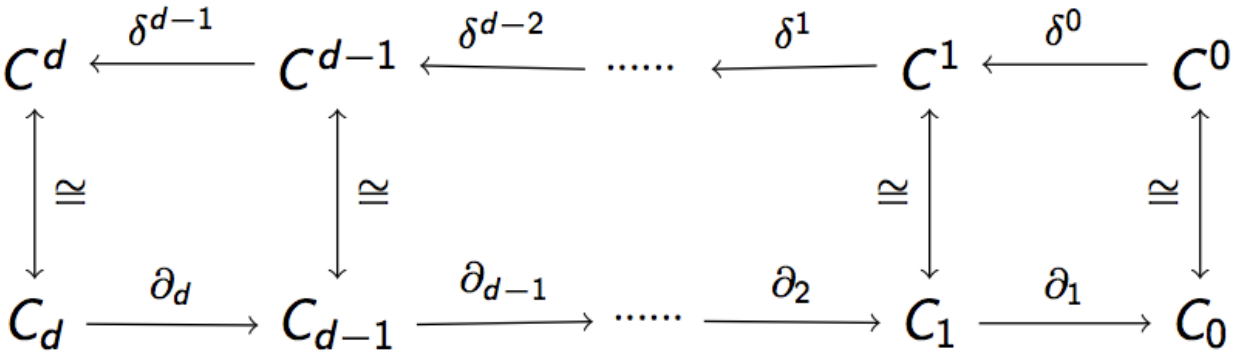
\includegraphics[width=0.75\linewidth]{images/chainComplexMap.png}\\
   \caption[Relationships between chains and cochains]{Relationships between chains and cochains}
   \label{fig:larComplexMap}
\end{figure}

At this point we are interested in computing these operators in an efficient way. As always, \cite{DiCarlo} provides an interesting algorithm based on the LAR representation schema. First of all, we should consider the incidence map $\ell_{p-1}^{p} \colon C_{p} \rightarrow C_{p-1}$ and its matrix $[\ell_{p-1}^{p}] = M^{p}_{p-1} = M_{p-1}M^{\mathsf{T}}_{p}$. The entry $M_{p-1}^{p}[i,j]$ stores the number $k$ of common vertices between the cells $\mu_{p-1}^{i}$ and $\lambda_{p}^{j}$, where $\mu \in \Lambda_{d-1}$ is the common facet between cell complexes and $\lambda \in \Lambda_{d}$ represents a single cell. In fact we have: $M^{p}_{p-1}[i,j] = \displaystyle\sum_{h=0}^{k_{0}-1} M_{p-1}[i,h] \cdot M_{p}[j,h] = \# (\mu_{p-1}^{i} \cap \lambda_{p}^{j}) = k$. So if we want to compute the \textbf{unoriented boundary} operator, we can use the following algorithm:

\begin{pseudo}[caption={Unoriented boundary algorithm}, label={lst:Boundary}]
begin
 $CSR(M_{p-1}^{p}) = CSR(M_{p-1})CSR(M_{p}^{\mathsf{T}})$
 foreach $i$ in $0 \leq i \leq k_{p-1} - 1$:
   $k = \#\mu_{p-1}^{i}$ //Number of nonzero elements for row $i$ of $CSR(M_{p-1})$
   foreach $j$ in $0 \leq j \leq k_{p} - 1$:
     if $M^{p}_{p-1}[i,j] = k$:
       $\partial_{p}[i, j] = 1$
     else:
       $\partial_{p}[i, j] = 0$
 return $\partial_{p}$
end       
\end{pseudo}

By duality, we can obtain the coboundary operator as the transposition of $\partial_{p}$ operator. For a better understanding of this algorithm we can see an example of $\partial_{2}$ computation from \cite{DiCarlo}. First of all we have to consider the cell complex in Figure~\ref{fig:boundaryExample} with the characteristic matrices $M_1$ and $M_2$.

\begin{figure}[htb] %  figure placement: here, top, bottom
   \centering
   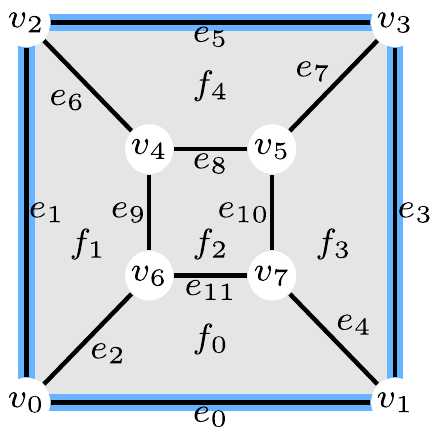
\includegraphics[width=0.35\linewidth]{images/boundaryExample.png}\\
   \caption[Cuboidal complex]{Cuboidal complex. Image taken from \cite{DiCarlo}}
   \label{fig:boundaryExample}
\end{figure}

According to the algorithm we have that $M_{1}^{2} = M_{1}M_{2}^{\mathsf{T}}$. So if:\\

$M_2 =
\begin{pmatrix}
1 & 1 & 0 & 0 & 0 & 0 & 1 & 1\\
1 & 0 & 1 & 0 & 1 & 0 & 1 & 0\\
0 & 0 & 0 & 0 & 1 & 1 & 1 & 1\\
0 & 1 & 0 & 1 & 0 & 1 & 0 & 1\\
0 & 0 & 1 & 1 & 1 & 1 & 0 & 0\\
1 & 1 & 1 & 1 & 0 & 0 & 0 & 0\\
\end{pmatrix}
M_1 =
\begin{pmatrix}
1 & 1 & 0 & 0 & 0 & 0 & 0 & 0\\
1 & 0 & 1 & 0 & 0 & 0 & 0 & 0\\
1 & 0 & 0 & 0 & 0 & 0 & 1 & 0\\
0 & 1 & 0 & 1 & 0 & 0 & 0 & 0\\
0 & 1 & 0 & 0 & 0 & 0 & 0 & 1\\
0 & 0 & 1 & 1 & 0 & 0 & 0 & 0\\
0 & 0 & 1 & 0 & 1 & 0 & 0 & 0\\
0 & 0 & 0 & 1 & 0 & 1 & 0 & 0\\
0 & 0 & 0 & 0 & 1 & 1 & 0 & 0\\
0 & 0 & 0 & 0 & 1 & 0 & 1 & 0\\
0 & 0 & 0 & 0 & 0 & 1 & 0 & 1\\
0 & 0 & 0 & 0 & 0 & 0 & 1 & 1\\
\end{pmatrix}$

we can obtain:\\

$M^{2}_{1} =
\begin{pmatrix}
2 & 1 & 0 & 1 & 0 & 2\\
1 & 2 & 0 & 0 & 1 & 2\\
2 & 2 & 1 & 0 & 0 & 1\\
1 & 0 & 0 & 2 & 1 & 2\\
2 & 0 & 1 & 2 & 0 & 1\\
0 & 1 & 0 & 1 & 2 & 2\\
0 & 2 & 1 & 0 & 2 & 1\\
0 & 0 & 1 & 2 & 2 & 1\\
0 & 1 & 2 & 1 & 2 & 0\\
1 & 2 & 2 & 0 & 1 & 0\\
1 & 0 & 2 & 2 & 1 & 0\\
2 & 1 & 2 & 1 & 0 & 0\\
\end{pmatrix}
\Rightarrow \partial_{2} = 
\begin{pmatrix}
1 & 0 & 0 & 0 & 0 & 1\\
0 & 1 & 0 & 0 & 0 & 1\\
1 & 1 & 0 & 0 & 0 & 0\\
0 & 0 & 0 & 1 & 0 & 1\\
1 & 0 & 0 & 1 & 0 & 0\\
0 & 0 & 0 & 0 & 1 & 1\\
0 & 1 & 0 & 0 & 1 & 0\\
0 & 0 & 0 & 1 & 1 & 0\\
0 & 0 & 1 & 0 & 1 & 0\\
0 & 1 & 1 & 0 & 0 & 0\\
0 & 0 & 1 & 1 & 0 & 0\\
1 & 0 & 1 & 0 & 0 & 0\\
\end{pmatrix}$